\begin{frame}
	\frametitle{clone}
	\begin{columns}
		\column{0.5\textwidth}
			\begin{itemize}
				\item <2-> alle Dateien werden in das working Directory kopiert
				\item <3-> alle remote Branches werden erstellt
				\item <4-> der default branche wird lokal erstellt (master)
			\end{itemize}	
		\column{0.5\textwidth}
			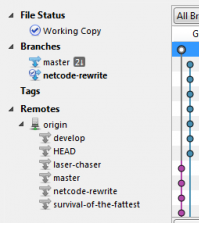
\includegraphics[scale=1.0]{./pictures/clone_branches}
	\end{columns}
\end{frame}
\begin{frame}
	\frametitle{clone}
	\begin{block} <1-> {Was benötigen wir zum clonen?}
		\begin{itemize}
			\item <1-> die URL, wo des remote repository liegt
			\begin{itemize}
				\item <1-> https://github.com/Lusito/GameDevWeek.git
			\end{itemize}
			\item <2-> einen lokalen Speicherplatz
		\end{itemize}
	\end{block}
\end{frame}
\begin{frame}
	\frametitle{clone}
	\centering {
		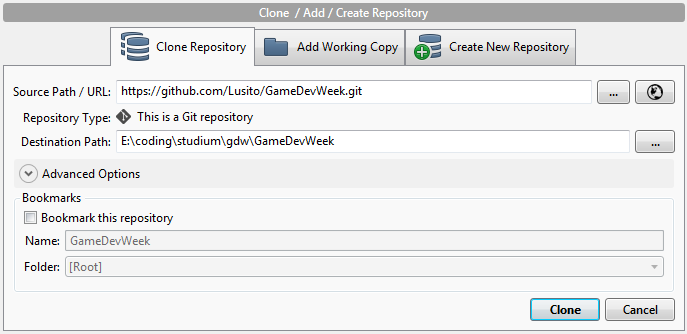
\includegraphics[scale=0.65]{./pictures/clone_sourceTree}
	}
\end{frame}